\documentclass[12pt]{article}

\usepackage[a4paper,top=2cm,bottom=2cm,left=2cm,right=2cm,marginparwidth=1.75cm]{geometry}

% Useful packages
\usepackage[affil-it]{authblk}
\usepackage{algorithm}
\usepackage{algpseudocode}
\usepackage{amsmath}
\usepackage{graphicx}
\usepackage[colorlinks=true, allcolors=blue]{hyperref}
\usepackage[
        backend=biber,
        style=authoryear,
        sorting=nyt,
    ]{biblatex}
\addbibresource{ref.bib} 
\usepackage{epigraph} % for quoting
\usepackage{float}
\usepackage{amsfonts}
\usepackage{caption}
\usepackage{array}
\usepackage{booktabs}
\usepackage[flushleft]{threeparttablex}
\usepackage{svg}
\svgsetup{inkscapelatex=false}
\usepackage{dcolumn}
\usepackage{tabularray}
\usepackage{longtable}
\usepackage{tablefootnote}

% \usepackage{longtable}

\title{If Inequality is an Economic Choice,\\What is the Relationship between Inequality and Growth?}


\author[1,+]{Khanh Duong}

\affil[1]{\small UNU-MERIT, Maastricht, The Netherlands}
\affil[+]{\small Corresponding author: duong@merit.unu.edu}


\date{} % This line hides the date

\begin{document}
\maketitle

\begin{abstract}
\noindent This study provides evidence that when economic development—encompassing both growth and inequality—is treated as an objective that benefits the entire economy rather than specific agents, growth and inequality can coexist and have a positive relationship. While some may be concerned that such a trade-off inevitably leads to extreme inequality that could hinder future growth, the findings indicate that this trade-off occurs within controlled bounds of inequality, as measured by a Gini index below 28. Although extending growth might suggest an increase in inequality, practical constraints and the inherent limits to growth prevent such extremes. The analysis utilises multi-objective optimisation, conceptualising both inequality and growth as policy objectives. The model identifies optimal strategies that maximise growth and minimise inequality within the observed range of GDP per capita, with deviations from these optimal choices interpreted as penalties reflecting non-economic factors. The results further support the hypothesis of a natural rate of subjective inequality.


\medskip
\textbf{Keywords:} Economic inequality, trade-offs, optimisation, natural inequality

\textbf{JEL Code:} D63, O10, O40, C61 

\end{abstract}
\newpage

\section{Introduction}

Economic development is a widely discussed yet poorly understood concept. Although development can be defined in different ways and from various perspectives, it is clear that it cannot only be reduced to economic growth as measured by GDP per capita. Development can also be understood in non-monetary terms, such as well-being or happiness \parencite{agrawal2024economic}. However, do we consider Bhutan, one of the happiest countries in the world, more developed than the United States? Or that hunter-gatherer societies, often described by \textcite{sahlins2013original} as among the most affluent societies, as more developed than contemporary ones? Development, in this case, represents a choice between growth and equality, as inequality helps explain the paradox between growth and happiness \parencite{oishi2015income}. There are trade-offs between growth and equality \parencite{okun2010equality}, as well as between monetary and non-monetary aspects of development \parencite{kahneman2010high}, and the former often determines the latter. For instance, humanity has historically moved away from an equal but impoverished existence in primitive societies to a wealthier, yet unequal current one. This progression aligns with the view that the United States is considered more developed than Bhutan, reflecting the dialectical notion that material conditions shape consciousness \parencite{lefebvre2009dialectical}. 

This paper will not delve too deeply into the broader definitions of development but will instead focus on monetary development, as it plays a decisive role. Monetary development is not limited to a narrow measure like GDP per capita. Assume development as described by a wealth (or income) distribution: GDP per capita represents its first moment (the mean value), while the inequality corresponds to its second moment (the variance). The two highest moments need not be explored, as inequality is sufficient as a major cause of social problems \parencite{neckerman2007inequality}, including climate change \parencite{duong2023does} and the socio-economic consequences of the pandemic \parencite{stantcheva2022inequalities}. To simplify development, growth and inequality are two sides of the same coin \parencite{berg2017inequality}. One might argue that this assumes a trade-off between growth and inequality \parencite{okun2010equality}, which remains a contested issue. For instance, the Kuznets curve suggests that beyond a certain threshold, growth and equality can coexist \parencite{nielsen1997kuznets}. Similarly, the concept of sustainable development advocates growth accompanied by reduced inequality \parencite{freistein2016potential}. This discussion is also related to the debate on whether inequality is a matter of choice \parencite{stiglitz2013inequality}. Namibia, for example, is often cited as a country that has successfully reduced inequality through deliberate policy interventions \parencite{lawson2017inequality}, providing a counterexample to the inevitability of inequality in the development process.

This study provides evidence supporting the argument that if development (growth and inequality) is an economic objective (that benefits the entire economy without favouring specific economic agents), then growth and inequality can coexist, indicating a positive relationship between the two. Some may worry that this trade-off would inevitably lead to extreme inequality, potentially hindering future growth \parencite{berg2017inequality}—an outcome that appears counter-intuitive. However, the findings in this paper show that the trade-off occurs with controlled inequality (a Gini index of less than 28). There is also concern that if growth were extended beyond observed data, inequality would escalate to extreme levels. However, it must be recognised that limits to growth \parencite{meadows2018limits} exist and practical constraints render such extreme values unachievable. The evidence presented here is based on multi-objective optimisation, where inequality and growth are treated as choices within the broader context of development. The model identifies optimal choices that maximise growth and minimise inequality within the observed range of GDP per capita data. Observed inequality may deviate from these optimal values, with penalties applied to reflect tolerance for inequality, influenced by non-economic factors such as fairness \parencite{cojocaru2014fairness}. These findings also support the ``natural rate of subjective inequality" hypothesis, as proposed by \textcite{lambert2003inequality}. 

\section{The theoretical background}
\subsection{The origins of economic inequality}

The origins of economic inequality have been the subject of significant philosophical, economic, and sociological inquiry, with various schools of thought offering differing explanations. From a historical standpoint, economic inequality can be traced to the emergence of agriculture and the rise of property ownership. In pre-agricultural societies, hunter-gatherers lived in relatively egalitarian conditions. However, the shift from a nomadic to a settled lifestyle with the advent of farming, around 10,000 years ago, allowed for surplus production and the accumulation of wealth. The control over land, resources, and food became central to societal power dynamics, leading to the formation of social hierarchies. This view is most famously articulated by Rousseau in his \textit{Discourse on the Origin of Inequality} \parencite*{rousseau1755}, where it was argued that private property was the root cause of social inequality. With the establishment of property rights, humans transitioned from a natural state of equality to a more structured and unequal society. The establishment of agricultural societies led to the division of labour, specialisation, and the accumulation of wealth by certain groups, thus institutionalising economic disparities.

Economic inequality is also closely tied to the formation and evolution of political systems. In the analysis of capitalist societies, Karl Marx \parencite*{marx1867} argued that economic inequality is intrinsically linked to the capitalist mode of production. According to Marx, the capitalist class (bourgeoisie) owns the means of production, while the working class (proletariat) sells their labour. This division between capital and labour creates an inherent structure of inequality, as the surplus value generated by workers is appropriated by capitalists, exacerbating wealth disparities. Max Weber \parencite*{weber1922}, in contrast, emphasised that inequality arises not only from economic factors but also from social stratification, including status and power. Weber argued that social classes are determined by a combination of economic position, social status, and political influence, which together produce and sustain inequality.

In contemporary economic discourse, inequality is often viewed through the lens of market structures, human capital, and technology. Economists like Thomas Piketty \parencite*{piketty2014capital}, in \textit{Capital in the Twenty-First Century}, argue that inequality in modern economies is driven by the rate of return on capital outpacing economic growth, leading to an increasing concentration of wealth. This phenomenon has been exacerbated by globalisation, financialisation, and changes in the labour market, where the rewards of capital have disproportionately gone to the wealthiest individuals, leaving labour's share of income stagnant or declining. The rise of automation and technological change has also contributed to the widening of inequality. The \textit{skill-biased technological change} hypothesis, for instance, suggests that advancements in technology disproportionately benefit highly skilled workers, exacerbating wage inequality \parencite{acemoglu2002technical}. Meanwhile, low-skilled workers face job displacement and stagnation in wages, further widening the economic divide. From a structural perspective, economic inequality is not merely a by-product of individual choices but is shaped by institutional and policy frameworks. For instance, inequality can be perpetuated by tax policies, education systems, and labour market regulations that favour wealthier individuals and corporations. The work of sociologists and economists such as \textcite{Pickett2009} highlights how the structure of income distribution within societies can impact a range of social outcomes, from health to education, reinforcing a cycle of inequality. 

\subsection{Inequality by-laws or choices}
This study revisits Rousseau's question regarding the ``state of nature" and its connection to the origins of economic inequality. Is the transition from a natural state of equality to a more structured and unequal society a matter of choice or an inevitable law? In this context, ``a law" refers to something beyond human control—more precisely, beyond government control. While political systems (linked to the state) and power systems are often seen as equivalent, they are, in fact, fundamentally different, with power systems being broader in scope. Power systems can be compared to the distribution of power in trade networks or firm sizes, independent of state intervention. These distributions may signify inherent laws, as they conform to the characteristics of the \textit{power-law distribution}. On the other hand, ``a choice" (referring to policy decisions) made under state control typically aims to achieve two outcomes: to benefit society as a whole (e.g., by promoting economic growth) and to benefit a select few (such as certain economic sectors, talented individuals, or holders of economic power). The latter is particularly evident when the state serves the interests of the ruling class. In such cases, the state effectively makes decisions that benefit a specific subpopulation rather than the entire nation, as Karl Marx argued. Even in today's democratic societies, this dynamic persists, as policy decisions can still disproportionately favour certain groups, such as corporations, wealthy individuals, or political elites.

To clarify the boundary between a law and a choice, two cases are presented, both without government intervention. The first case is a study on species abundance inequality of the most common tree species in the Amazon rainforest by \textcite{scheffer2017inequality}. Interestingly, they found similarities with wealth inequality in human societies, with both following a power-law distribution. Specifically, the global wealth distribution among 1,800 billionaires shows extreme concentration at the top, with a small number controlling most of the wealth. Similarly, the abundance of tree species in the Amazon is dominated by a few species, with most species being far less common. Additionally, the Gini index of wealth across countries highlights economic inequality, with wealth concentrated in a few nations. Similarly, the Gini index of species abundance reveals a few species dominating ecosystems, indicating unequal distribution within natural communities. This may suggest that the natural inequality Rousseau referred to could be significant; however, it is important to carefully interpret these findings, as resource distribution within a species tends to be relatively equal, which is not the same as the significant inequality found within human societies. 

The second case is a study of wealth inequality by \textcite{fuchs2014behavioral} in the virtual world of massively multiplayer online games (MMOGs), where players engage in complex economic activities such as trade, production, and accumulation of social status. Some of these virtual worlds have populations that exceed those of small countries; thus, these worlds can be viewed as counterparts to real-world countries with free-market systems, characterised by minimal government intervention. Research on wealth inequality in these virtual environments demonstrates patterns akin to the wealth distribution data from Sweden (2007) and the UK (2005), where the wealth distribution manifests a power-law tail, while the middle segment is more accurately represented by an exponential distribution. The Gini index of wealth distribution in these virtual worlds is 0.653, which approximates the wealth inequality observed in Germany in 1998 (Gini = 0.667) and the UK in 2000 (Gini = 0.697). It is also relatively close to the Gini index of a Gaussian distribution (Gini = 0.636). These findings suggest that inequality is moulded by similar principles in both nature and society. Nonetheless, it is important to acknowledge that both natural and virtual worlds do not possess the same considerations for humanity and welfare that human societies exhibit.

As presented here, if economic inequality resulting from inevitable laws is relatively high (Gini = 0.653), then the portion of inequality driven by political choices is approximately 0.236 - which represents the difference between the global wealth inequality in 2021 (Gini = 0.889), as reported by Credit Suisse \parencite{suisse2022global}, and the inequality attributed to inevitable laws. While inequality can be shaped by political decisions, it is not inherently detrimental.  According to the \textit{Marginal Propensity to Save} theory, wealthier individuals tend to save a larger share of their income compared to those with lower wealth, primarily due to the higher returns they receive on their relatively less risky assets \parencite{fagereng2020heterogeneity}. Although this argument oversimplifies the issue and has notable limitations, it aligns with the widely accepted view that some degree of inequality is necessary. In fact, moderate inequality can incentivise competition and innovation \parencite{balietti2021incentives}. Empirical evidence suggests that countries with relatively low inequality in pay structures—such as those in Scandinavia—consistently exhibit higher productivity and lower unemployment rates than their more unequal counterparts \parencite{galbraith2016inequality}. However, for inequality to contribute positively to economic outcomes, it must be accompanied by fairness and institutional trustworthiness.  As argued above, political choices (or policy decisions) can either benefit the broader economy—without necessarily increasing inequality—or primarily benefit a privileged few, thereby exacerbating inequality. Since the focus here is economic inequality, political choices that support the whole economy are referred to as ``economic purpose" and those that disproportionately favour a select group as ``bias purpose". Accordingly, this study aims to address the following question:  
\begin{quote}
If inequality is an economic choice without bias purposes, what is the relationship between inequality and growth?
\end{quote}

\begin{figure}[H]
\centering
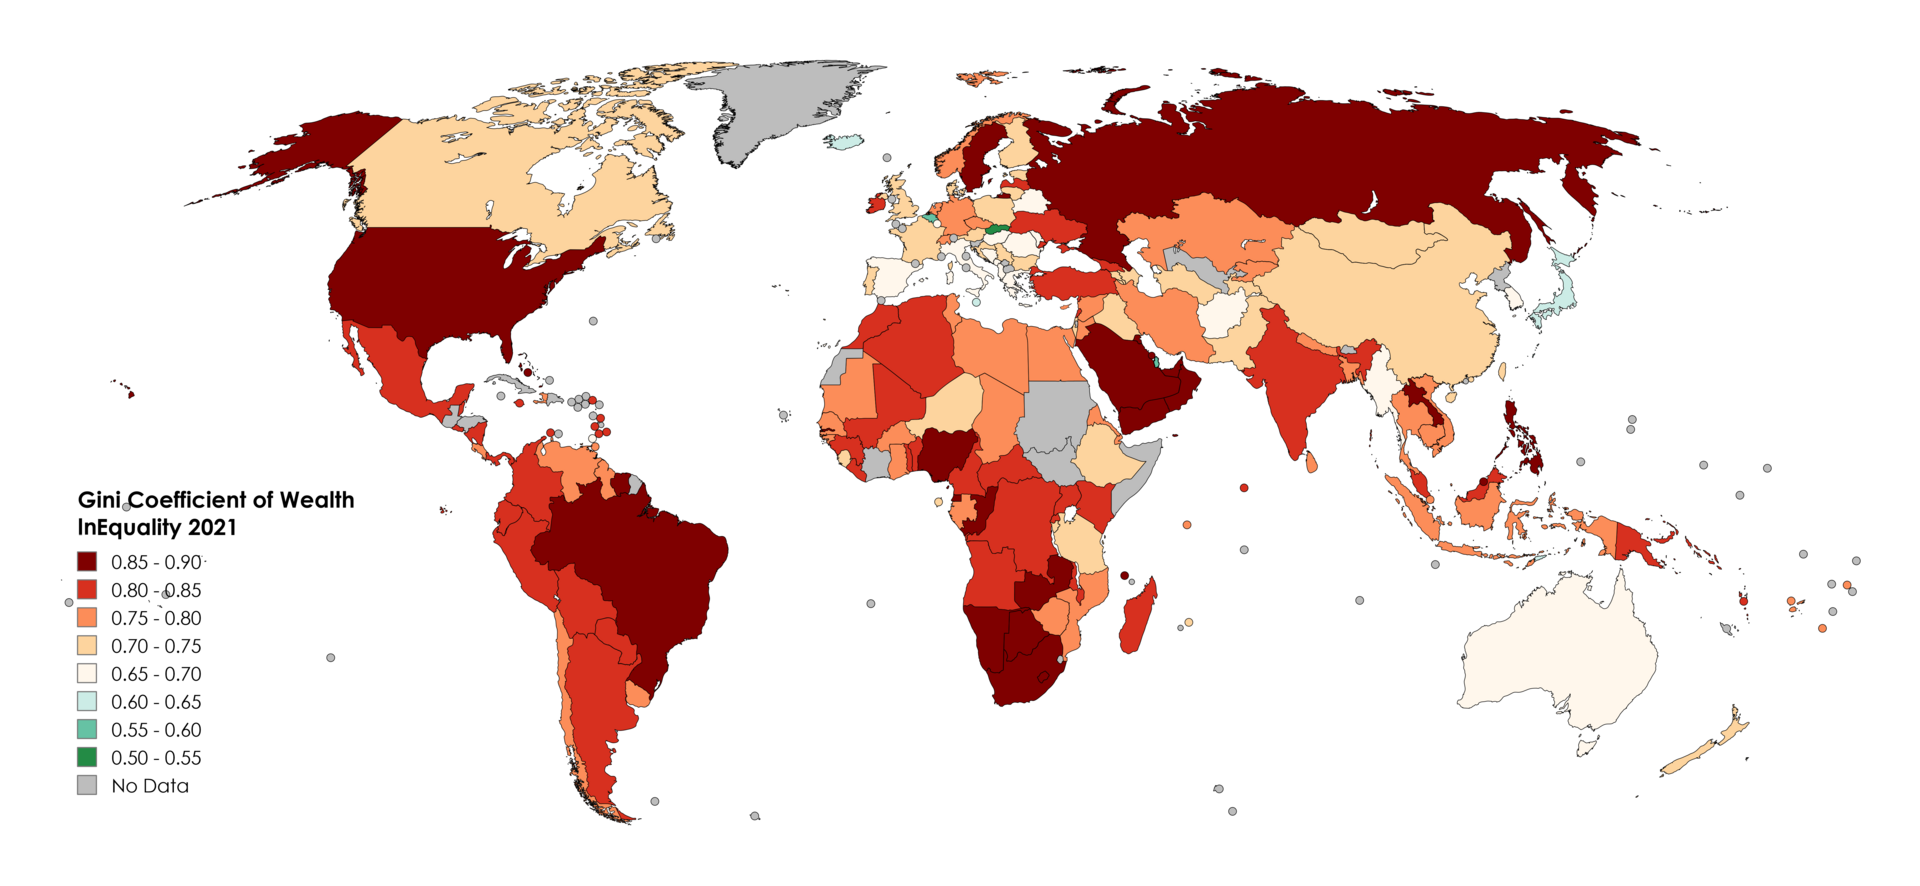
\includegraphics[width=1\linewidth]{figs/global_wealth_distribution.png}
\caption{Global Wealth Inequality 2021}
\captionsetup{font=footnotesize}
\caption*{\textbf{Notes:} Calculations are based on a total of 5,298,564 thousand adults, with an average wealth per adult of 87,489 USD. The estimated global wealth Gini coefficient is 88.9.\\
Source: Credit Suisse Global Wealth Databook \parencite*{suisse2022global}}
\end{figure}

\section{Data and methods}

\subsection{Data and variables} \label{sec:data}

\textit{Measurement of outcomes:} This study focuses on income inequality as the most relevant measure of economic disparity, as it directly reflects the distribution of monetary resources within a country. This aligns with the definition of monetary development as the distribution of income. Unlike pay inequality, which captures disparities in wages and salaries from labour market earnings, income inequality encompasses a broader range of income sources, including wages, capital income, and government transfers, making it a more comprehensive measure of economic distribution. While wealth inequality tends to be more persistent and extreme, it primarily reflects accumulated assets and intergenerational transfers rather than the immediate income flow that determines economic access and opportunities in the short term. Given that this study examines the first two moments of the income distribution—mean income (GDP per capita) and variance (the Gini Index of disposable income)—income inequality is the appropriate focus, as it captures both the overall level of economic resources and their dispersion within society.  

This study measures income inequality using data from the Luxembourg Income Study (LIS) and the Standardised World Income Inequality Database (SWIID), balancing reliability with coverage. LIS is the most reliable source, providing harmonised micro-data from household surveys that allow for consistent measurement of both market and disposable income inequality. However, its main limitation lies in its limited country and time coverage. On the other hand, SWIID offers the widest coverage by standardising data from various sources and employing imputation techniques to fill gaps. As highlighted by \textcite{galbraith2014utip}, a key issue with SWIID is that it distorts market inequality in wealthier countries due to its reliance on public pensions, which skews comparisons with more unequal nations. Additionally, Solt's imputation method for deriving disposable income measures may lead to cases where the redistribution gap is not independent. The primary findings of this study are based on LIS, due to its higher data quality, while SWIID is used for robustness checks to ensure that the results are not influenced by data limitations. By combining these datasets, the study ensures both analytical depth and broader applicability in examining income inequality and distribution.

\textit{Measurement of predictors:} Economic choice of inequality is defined as policy decisions that enhance overall economic outcomes without granting biased advantages to specific groups of economic agents. In the economic domain, when variables are quantified and incorporated into a function to determine optimal outcomes, economic choices resemble an optimisation rule rather than a deliberate trade-off between incomparable options. To achieve this, economic considerations are made at the national level, economic choice is defined as one that benefits the entire nation, and these considerations are structured into an optimal function for monetary development outcomes. Key factors in this process include globalisation, technology, economic instability, fertility, taxation, education, and financialisation. While these factors may not comprehensively capture all economic dynamics, they represent the core elements of economic considerations in formulating a development strategy, as discussed in contemporary economic theory. 

\begin{itemize}
    \item \textit{Globalisation}: While emerging economies have leveraged globalization and technology for growth, these forces have also widened inequality. Trade-led growth can reduce disparities \parencite{jaumotte2013rising}, but FDI-driven expansion often increases wage gaps by raising skill premiums \parencite{Eichengreen2021}. Labour-saving and skill-biased technologies further exacerbate inequality by displacing workers \parencite{acemoglu2019automation}. Although globalization is frequently blamed for rising inequality \parencite{ravallion2018inequality}, some argue that technological change is the primary driver \parencite{furceri2019robust}. Trade globalization may reduce inequality, while financial globalization tends to worsen it \parencite{asteriou2014globalization}. However, distinguishing their effects remains challenging, as they are deeply interconnected \parencite{davis2018fourth}.
    \item \textit{Technology}: Long regarded as a key driver of economic growth, its impact on inequality remains inconclusive. Samuelson \parencite*{Samuelson1964} and Solow \parencite*{Solow1956, Solow1957} argued in their neoclassical growth model that technological progress universally raises wages by enhancing productivity. However, the skill-biased technological change hypothesis faces empirical challenges. Galbraith \parencite{galbraith1998created} and Howell \parencite*{Howell1996} question its validity, citing the weak correlation between IT diffusion and rising inequality in the U.S. Additionally, despite the increased demand for skilled workers, productivity growth stagnated in the 1980s, contradicting expectations \parencite{Rosenberg1982}. While some contend that technological shifts require time to reshape labour markets, this delay does not fully account for the observed trends \parencite{galbraith2016inequality}.
    \item \textit{Credit:} \textcite{galor1996income} present a general equilibrium model that extends the Kuznets hypothesis by making growth and inequality endogenous. The model explains the inverted-U relationship through capital market imperfections, where borrowing requires collateral, disadvantaging the poor. During early development, investment primarily benefits high-income groups, leading to rising inequality. However, as growth progresses, opportunities for the poor improve, enabling higher returns on their investments. The persistence of inequality, however, hinders growth by reducing overall investment levels. This revised mechanism underscores a negative causal link between inequality and growth, a concept that has gained considerable empirical support in recent literature.
    \item \textit{Redistribution:} One factor directly linked to the relationship between growth and inequality is redistribution. According to \textcite{alesina1994distributive} and \textcite{NBERw5658}, greater inequality increases voter demand for redistributive policies. These policies, typically characterised by higher taxation, can lead to inefficiencies by discouraging effort, entrepreneurship, and investment. As a result, economic growth may slow due to suboptimal resource allocation and reduced incentives for productive activity. These models underscore the trade-offs between redistribution and growth, demonstrating how political responses to inequality can have unintended negative consequences on the overall economy.
    \item \textit{Human capital:} The neoclassical growth model's treatment of human capital, as outlined by \textcite{Becker1993, Schultz1960}, assumes that human capital is merely another form of capital that is smoothly substitutable across varying levels of education and skill. This perspective preserves the inherent complementarity between labour and technology in the production function. As a result, the model does not provide a mechanism for technological progress to differentially affect the wages of workers based on their qualifications. Consequently, wage disparities stemming from technological change are absent in these frameworks, limiting their explanatory power regarding observed inequalities linked to technological advancements.
    \item \textit{Fertility:} The implications of fertility rates are significant for both economic growth and inequality \parencite{de2003inequality}. High fertility rates, especially when they vary across income groups, can exacerbate inequality. In societies where wealthier individuals have fewer children, resources and human capital become concentrated within certain segments of the population, leading to greater economic disparities. This differential fertility can also affect economic growth, as a high degree of inequality can limit broader economic opportunities and reduce overall growth prospects. While some level of inequality may stimulate investment and innovation, the concentration of wealth within a small group can restrict social mobility and the potential for sustainable growth.
    \item \textit{Instability:} Monetary development, encompassing growth and inequality, is closely linked to instability through inflation and unemployment \parencite{rolim2024inflation}. High inequality can drive inflation, as distribution conflicts between capital and labour lead to rising costs that undermine investment and growth. Economies with more equitable income distribution tend to experience more stable inflation, supporting sustainable growth. On the labour side, inequality contributes to unemployment by causing mismatches in the labour market, as workers migrate for better opportunities. Inequality also limits aggregate demand, hindering job creation. Evidence shows that countries with lower inequality, like those in Scandinavia, experience higher productivity and lower unemployment, promoting stability and growth \parencite{galbraith2016inequality}. Therefore, reducing inequality is essential for both economic stability and long-term development.
\end{itemize}

The dataset used in this study is a comprehensive cross-country, cross-time panel that integrates various sources of economic indicators. It includes data from the Luxembourg Income Study (LIS), the Standardised World Income Inequality Database (SWIID), the Penn World Table (PWT), and World Bank indicators. These datasets span multiple years and countries, and after merging, they are harmonised by country and year. A list of the countries included in this study is provided in Table \ref{tab:country} in the Appendix. Descriptive statistics of the original data are presented in Table \ref{tab:descriptive_original} (Appendix). To ensure data quality and completeness, observations with missing values in key outcomes—GDP per capita and disposable income inequality—are excluded. The imbalance between countries and years is illustrated in Figure \ref{fig:panel} in the Appendix.

\begin{table}[H]
\centering
\footnotesize
\renewcommand{\arraystretch}{1.5} % Increase row height
\caption{Variables, Descriptions, and Data Sources}
\label{tab:var}
\begin{tabular}{|p{2cm}|p{3cm}|p{7cm}|l|}
\hline
\textbf{Type} & \textbf{Variables} & \textbf{Description} & \textbf{Data Source} \\
\hline
\textbf{Outcome} & GDP per capita & GDP per capita in constant 2015 US\$. & World Bank \\
\cline{2-4}
& Gini Index & Gini index of disposable income, measuring income inequality. & LIS/SWIID\\
\hline
\textbf{Predictors} & Redistribution & Difference between market income Gini and disposable income Gini, reflecting the impact of redistributive policies.& LIS/SWIID\\
\cline{2-4}
& Human Capital & Educational attainment and quality. & PWT \\
\cline{2-4}
& Technology & Total factor productivity, capturing innovation and skills. & PWT \\
\cline{2-4}
& Trade & Trade as a percentage of GDP. & World Bank \\
\cline{2-4}
& FDI & FDI net inflows as a percentage of GDP. & World Bank \\
\cline{2-4}
& Credit & Domestic credit to the private sector as a percentage of GDP. & World Bank \\
\cline{2-4}
& Fertility & Total births per woman (fertility rate). & World Bank \\
\cline{2-4}
& Unemployment & Unemployment rate as a percentage of the total labour force (using ILO modelled estimates). & World Bank \\
\cline{2-4}
& Inflation & Annual percentage change in consumer prices. & World Bank \\
\hline
\end{tabular}
\vspace{0.2cm}
\captionsetup{font=footnotesize}
    \caption*{\textbf{Notes:} LIS stands for Luxembourg Income Study, SWIID stands for Standardised World Income Inequality Database, PWT refers to the Penn World Table, FDI means Foreign Direct Investment, GDP is Gross Domestic Product, and ILO stands for the International Labour Organization. The data has been extracted and is current as of November 2024, reflecting the most recent updates available.}
\end{table}

Furthermore, several exclusions that lie outside the scope of economic choices are highlighted, as they are not driven by deliberate decision-making based on economic rationality. First, path dependency in development is discussed, where growth and inequality are shaped by historical trajectories and time-varying effects. This includes the persistence of past values over time, rather than intentional decisions. Path dependence creates self-reinforcing cycles from early choices—such as technology adoption or industry location—that are difficult to alter, ultimately widening inequality and fostering divergent growth paths \parencite{david1985clio, atolia2012growth, halter2014inequality}. Early decisions in productivity and structural changes further exacerbate inequality. Second, political institutions are addressed, which allocate power and resources but are influenced by entrenched interests rather than economic considerations. These institutions shape growth and inequality by determining resource distribution, with inclusive institutions promoting equity and growth, while extractive ones concentrate power, perpetuating inequality. Even in democracies, elite influence can limit redistributive policies \parencite{acemoglu2001colonial, gilens2012affluence}. Additionally, the legacy of colonialism is considered, with historical and systemic impacts—including time-varying institutional effects—that continue to affect growth and inequality without being the result of contemporary economic decisions. Colonial powers established governance systems that benefited colonizers and created institutional structures in post-colonial nations, reinforcing inequality \parencite{NBERw11057, cypher2014development}.

\subsection{Analytical methods}

To address missing values in the predictor variables (excluding the outcome variables) and standardize their scale, the dataset undergoes preprocessing steps, which include imputation and normalisation. Missing data are addressed using \textit{bagged imputation}, which employs an ensemble of predictive models trained on bootstrapped subsets of the data. Specifically, for a variable \(x_j\) with missing entries, \(B\) bootstrapped datasets are generated, and a predictive model \(f_b(x)\) is trained on each bootstrapped subset. The missing value for a given observation \(i\) is predicted as the average output of these models, mathematically represented as:

\[
\hat{x}_{ij} = \frac{1}{B} \sum_{b=1}^{B} f_b(\mathbf{X}_{-j,i}),
\]
where \(\mathbf{X}_{-j,i}\) represents the non-missing predictors for observation \(i\), excluding the missing value \(x_j\). This ensemble approach mitigates the risk of overfitting and improves robustness by aggregating multiple predictions from different models. 
Once imputation is complete, the variables are \textit{normalised} to a scale of \([0, 1]\) to facilitate comparability and improve the stability of subsequent analyses. The normalisation is achieved by applying the following formula to each variable \(x_j\):

\[
x_j^{\text{norm}} = \frac{x_j - \min(x_j)}{\max(x_j) - \min(x_j)},
\]
where \(\min(x_j)\) and \(\max(x_j)\) represent the minimum and maximum observed values of the variable \(x_j\), respectively. This transformation ensures that all normalised values \(x_j^{\text{norm}}\) fall within the interval \([0, 1]\), irrespective of the original scale of \(x_j\). Normalisation is crucial for ensuring comparability when variables are measured in different units, preventing those with larger magnitudes from dominating the model. It also enhances numerical stability and facilitates faster convergence during optimisation by keeping the predictor values bounded within a consistent range. The descriptive analysis of the cleaned data is shown in Table \ref{tab:descriptive_normalised} (see the Appendix).

Following the pre-processing, the analysis employs a multistep framework that integrates \textit{Elastic Net regression} and \textit{multi-objective optimisation} to identify the optimal trade-offs between maximising GDP per capita growth and minimising income inequality, as measured by the Gini index. The predictors for this analysis include redistribution, human capital, technology, trade, foreign direct investment (FDI), credit, fertility, unemployment, and inflation. The Elastic Net regression technique is applied to address the problem of \textit{multicollinearity}, a common issue when predictors are highly correlated, which can lead to unstable and unreliable coefficient estimates. Elastic Net combines both Lasso (\(L_1\)) and Ridge (\(L_2\)) regularisation techniques, shrinking the coefficients and selecting relevant variables simultaneously. This improves the interpretability and predictive performance of the model. The Elastic Net objective function is defined as:

\[
\hat{\beta} = \arg \min_{\beta} \left[ \sum_{i=1}^{n} \left( y_i - \mathbf{X}_i \beta \right)^2 + \alpha \sum_{j=1}^{p} \beta_j^2 + (1-\alpha) \sum_{j=1}^{p} |\beta_j| \right],
\]
where \(y_i\) represents the response variable (either GDP growth or income inequality), \(\mathbf{X}_i\) is the vector of predictors for observation \(i\), \(\beta_j\) are the model coefficients, and \(\alpha\) is a hyperparameter that controls the balance between the Ridge and Lasso penalties. To ensure optimal performance, the model is trained using \textit{5-fold cross-validation}, and the value of \(\alpha\) is selected based on the lowest Root Mean Squared Error (RMSE). 

The research objective is to determine the optimal values independently of the constraints imposed by specific national contexts, including political institutions and inevitable laws influenced by factors such as time- or path-dependency. Therefore, the goal is to isolate the effects of economic predictors from country- and time-related effects, rather than focusing on goodness-of-fit. Since country and time effects are not accounted for in the models, they will be captured in the residuals. Hence, ensuring no endogeneity in both models is necessary, meaning that residuals are uncorrelated with predictors (see Table \ref{tab:endo} in the Appendix). Another point to note is that coefficients act as weights in the optimization process by decision factors (or predictors), and such weights may be distorted by multicollinearity. Therefore, Elastic Net will help address this issue. It is also important to note that total causal effects are not required, but direct effects are considered in the simultaneous examination of economic predictors, as outlined in the estimation method of this study. Once the coefficients are estimated through Elastic Net, they are used to construct the \textit{objective functions} for GDP growth and inequality. These functions are defined as:

\[
\text{Growth} = \sum_{j=1}^{p} \beta_{j}^{\text{growth}} \cdot x_j; \text{Inequality} = \sum_{j=1}^{p} \beta_{j}^{\text{inequality}} \cdot x_j
\]
where \(\beta_{j}^{\text{growth}}\) and \(\beta_{j}^{\text{inequality}}\) are the coefficients corresponding to GDP growth and inequality, respectively, and \(x_j\) represents the normalised predictor values. The \textit{growth objective} is negated to facilitate maximisation, while the \textit{inequality objective} is directly minimised.

To balance the competing objectives, the analysis employs \textit{NSGA-II (Non-dominated Sorting Genetic Algorithm II)}, an evolutionary multi-objective optimisation algorithm widely utilised for addressing complex, conflicting optimisation problems \parencite{deb2002fast}. NSGA-II aims to find a set of \textit{Pareto-optimal solutions}, where no solution can improve one objective without worsening the other. The algorithm proceeds as follows:

\begin{enumerate}
    \item \textbf{Initial Population:} A random population of candidate solutions is generated, where each solution corresponds to a set of predictor values \( \mathbf{x} = [x_1, x_2, \dots, x_p] \).
    \item \textbf{Non-dominated Sorting:} Solutions are ranked based on their dominance. A solution \(x_i\) dominates another solution \(x_j\) if it performs at least as well in all objectives and strictly better in at least one objective. Solutions are grouped into \textit{fronts} based on dominance, with the first front containing the best solutions.
    \item \textbf{Crowding Distance:} Within each front, a \textit{crowding distance} is assigned to each solution. This distance measures how close a solution is to its neighbours in the objective space. Solutions with higher crowding distances are preferred, as they help maintain diversity in the population.
    \item \textbf{Selection:} The tournament selection process is used, where two solutions are randomly selected, and the one with the better rank (higher dominance) is chosen. If both solutions are in the same rank, the one with the higher crowding distance is selected.
    \item \textbf{Crossover and Mutation:} Genetic operators are applied to selected solutions. \textit{Crossover} combines two solutions, creating offspring that inherit characteristics from both parents. \textit{Mutation} introduces random changes to offspring, ensuring genetic diversity and the exploration of new regions of the solution space.
    \item \textbf{Elitism:} The best solutions from both the parent and offspring populations are retained. This ensures that the best solutions are preserved, preventing the loss of high-quality solutions during the evolutionary process.
    \item \textbf{Termination:} The algorithm iterates through the process of selection, crossover, mutation, and elitism until a stopping criterion is met—typically when the solutions converge to a stable Pareto front or a predefined number of generations is reached.
\end{enumerate}

The final result of the NSGA-II algorithm is a \textit{Pareto front}, which visualises the trade-offs between higher GDP growth and reduced income inequality. Each point on the Pareto front represents a policy combination where improving one objective (e.g., GDP growth) would result in a trade-off with the other (e.g., income inequality). This Pareto front provides policymakers with a set of optimal policy options that balance these competing goals.


\section{Results and discussion}

\textcite{berg2017inequality} argue that ``over longer horizons, avoiding excessive inequality and sustaining economic growth may be two sides of the same coin.'' This suggests that reducing excessive inequality can contribute to more sustainable economic growth over time. However, it is crucial to distinguish excessive inequality from moderate, controlled increases in inequality, just as sustainable growth differs from short-term or general economic growth. Therefore, this statement should not be simplistically interpreted as implying that greater equality and greater growth always go hand in hand. By contrast, Okun \parencite*{okun2010equality} famously stated, ``the money must be carried from the rich to the poor in a leaky bucket. Some of it will simply disappear in transit, so the poor will not receive all the money that is taken from the rich.'' This illustrates the efficiency-equity trade-off, where policies aimed at maximising efficiency (e.g., market mechanisms, deregulation, or productivity enhancements) may lead to greater inequality, whereas those prioritising equity (e.g., redistribution, social welfare programmes) may reduce incentives for economic efficiency. This growth-inequality relationship appears to contradict the argument made by \textcite{berg2017inequality}. However, Okun's trade-off primarily concerns redistribution and does not necessarily apply to cases where weak institutions result from high levels of inequality.

Evidence from the Luxembourg Income Study (LIS) dataset (see Figure \ref{fig:trend}) indicates that the most egalitarian countries (blue line) tend to be affluent, whereas poorer nations (red line) exhibit higher inequality. The red line, consistent with the argument of \textcite{berg2017inequality}, represents poorer countries (GDP per capita in constant 2015 USD $<$ 23,026) and shows a sharp decline in inequality as income rises, contradicting the Kuznets Curve \parencite*{kuznets1955economic}. For example, several Latin American countries have seen reductions in inequality alongside economic growth. The high levels of inequality and low growth in the region are often attributed to weak institutions \parencite{undp2021trapped}, which stem from colonialism \parencite{coatsworth2008inequality}. As a result, strengthening institutions could be key to addressing both inequality and growth challenges. Conversely, the blue line, which aligns with Okun’s major trade-off hypothesis, indicates a minor rise in inequality in wealthy, low-inequality nations (Gini $<$ 28) as their incomes increase, a trend frequently seen in advanced European economies. This suggests that technological progress disproportionately benefits higher-income groups, thereby exacerbating disparities. These trends align with the Augmented Kuznets Curve \parencite*{conceicao2001toward}, which incorporates additional factors such as technology and globalization. In poorer countries (red line), the decline in inequality reflects progress beyond early industrialization, driven by improvements in education, labour market reforms, and redistributive policies. Conversely, in affluent countries (towards the right side of the blue line), rising inequality underscores the impact of skill-biased technological change and globalization, which tend to favour high-skilled workers and capital owners.

\begin{figure}[H]
    \centering
    \scalebox{0.65}{\includesvg{figs/trends.svg}}
    \caption{Normalised Income and Inequality}
    \label{fig:trend}
    \captionsetup{font=footnotesize}
    \caption*{\textbf{Notes:} The chart shows the relationship between income (GDP per capita) and inequality. Each data point represents the mean income and inequality for a country over all time periods. The red line indicates a linear trend for data points where normalised income is less than 0.2 (or GDP per capita in constant 2015 USD $<$ 23,026), and the blue line indicates a linear trend for data points where normalised inequality is less than 0.2 (or Gini $<$ 28). The data is normalized and sourced from the LIS dataset and WDI, collected in November 2024.}
\end{figure}


To investigate the relationship between economic growth (GDP per capita) and income inequality as outcomes of economic choices, multi-objective optimisation is applied to maximise growth while minimising inequality. This analysis incorporates key economic factors, such as globalisation, technology, economic instability, fertility, taxation, education, and financialisation (as detailed in Section \ref{sec:data}). The optimal values for growth and inequality (as the Pareto Front output) are estimated using either the LIS dataset (for the primary results, shown in Figure \ref{fig:lis}) or the SWIID dataset (for robustness, shown in Figure \ref{fig:swiid}). The findings reveal a positive linear relationship between optimal growth and inequality, with results validated through a population size exceeding 1,000 and tested across multiple random seed iterations. The robustness of this result holds across both datasets—LIS (the most reliable) and SWIID (which offers broader coverage). This relationship resembles the trade-off between efficiency (GDP per capita) and equity (Gini index of disposable income) identified by \textcite{andersen2020big}. Their study employs stochastic frontier analysis to examine this trade-off across 33 OECD countries from 1970 to 2014, using the SWIID. The authors argue that while countries like the USA and Sweden have experienced increasing inequality, this shift is largely a result of movement along the frontier, leading to greater efficiency at the expense of equity.

Figure \ref{fig:lis}, based on the LIS dataset, demonstrates that as GDP per capita increases, income inequality also rises. The Pareto Front output (orange points) highlights this trend across 1,299 observations, showing a strong and highly significant correlation. The model explains nearly all variations in inequality, reinforcing the notion that economic growth tends to be accompanied by increasing income disparities. A similar pattern appears in Figure \ref{fig:swiid}, which uses the SWIID dataset, derived from a broader sample of 4,084 Pareto Front output pairs. Although the relationship is slightly weaker, it remains highly significant, confirming that inequality generally rises alongside income growth. These findings suggest that if inequality results from economic choices, an increase in income may lead to a modest rise (approximately 10\%) in income inequality.  This implies that even in the absence of biased policy decisions, economic policies that benefit overall growth may still contribute to a controlled increase in income inequality. However, this should not necessarily be interpreted as a big trade-off between efficiency and equity, given that the estimated slope is only around 0.1.

\begin{figure}[H]
    \centering
    \scalebox{0.6}{\includesvg{figs/Lis.svg}}
    \caption{Trade-off between growth and inequality choices using LIS}
    \label{fig:lis}
    \captionsetup{font=footnotesize}
    \caption*{\textbf{Notes:} Each data point represents the income (GDP per capita) and inequality for a specific country in a specific year.  The Pareto Front output (the orange points) reveals a strong positive relationship between GDP per capita and inequality for 1299 observations, with a coefficient of 0.1349 (\( p < 2 \times 10^{-16} \)). The model explains approximately 100\% of the variance in inequality (\( R^2 \approx 1 \)), with a residual standard error of \( 4.536 \times 10^{-6} \). The F-statistic is \( 1.311 \times 10^9 \) (\( p < 2.2 \times 10^{-16} \)), indicating a highly significant model.}
    \label{fig:trade_off}
\end{figure}


This can be attributed to the idea that inequality promotes competition, innovation, and productivity in fair and just societies such as Luxembourg (LUX), Norway (NOR), Denmark (DNK), Sweden (SWE), and the Netherlands (NLD), as shown in Figures \ref{fig:lis} and \ref{fig:swiid}. In other words, a modest increase in income inequality in an already relatively equal society may be a necessary and natural consequence of economic development. To illustrate this, the blue-dashed trend line is plotted based on the slope of the Pareto Front output, which shares the same right-hand intercept as the blue line in Figure \ref{fig:trend}. This intercept occurs at income = 1, rather than income = 0, as the blue line better represents affluent societies. The gap between the Pareto Front output and the blue-dashed trend line is what is termed the ``inequality penalty,'' as it is explained by non-economic factors. The findings may also suggest the natural rate of subjective inequality, as proposed by \textcite{lambert2003inequality}. The ``natural rate of subjective inequality" hypothesis posits that countries could, in theory, organise their affairs to achieve the same level of subjective inequality, meaning they would be willing to give up the same percentage of income to reduce inequality without affecting overall welfare (in a welfare-neutral way). However, in practice, countries differ in their degree of inequality aversion—how much inequality they are willing to tolerate. These differences in inequality aversion result in varying levels of objective inequality (e.g., the Gini coefficient) across countries. Countries with higher inequality aversion would redistribute more, leading to lower inequality, while those with lower aversion would tolerate higher inequality.

\begin{figure}[H]
    \centering
    \scalebox{0.6}{\includesvg{figs/Swiid.svg}}
    \caption{Trade-off between growth and inequality choices using SWIID}
    \label{fig:swiid}
    \captionsetup{font=footnotesize}
    \caption*{\textbf{Notes:} Each data point represents the income (GDP per capita) and inequality for a specific country in a specific year. The Pareto Front output (the orange points) shows a significant positive relationship between GDP per capita and inequality for 4084 observations, with a coefficient of 0.0778 (\( p < 2 \times 10^{-16} \)). The model explains 98.63\% of the variance in inequality (\( R^2 = 0.9863 \)), with a residual standard error of 0.00185. The F-statistic is \( 2.931 \times 10^5 \) (\( p < 2.2 \times 10^{-16} \)), indicating a highly significant model.}
\end{figure}

\section{Conclusion} 

In conclusion, the analysis demonstrates that economic inequality emerges from both natural laws and political choices. On one hand, evidence from studies of species abundance in the Amazon rainforest \parencite{scheffer2017inequality} and wealth distribution in virtual economies \parencite{fuchs2014behavioral} underscores that fundamental processes—exemplified by power-law distributions—can generate substantial inequality independent of governmental intervention. On another hand, the multi-objective optimisation results, derived from robust datasets such as the Luxembourg Income Study (LIS) and the Standardised World Income Inequality Database (SWIID), reveal a positive and highly significant relationship between GDP per capita and income inequality. This indicates that even in the absence of overtly biased policy decisions, economic growth is naturally accompanied by a modest increase in inequality—a finding consistent with the Augmented Kuznets Curve \parencite{conceicao2001toward} and the natural rate of subjective inequality hypothesis \parencite{lambert2003inequality}. Furthermore, empirical evidence suggests that while some degree of inequality may stimulate competition, innovation, and productivity \parencite{balietti2021incentives}, excessive inequality—especially when driven by politically motivated, biased policies—could undermine broader economic welfare \parencite{galbraith2016inequality}. Therefore, policymakers must carefully balance economic growth objectives with redistributive measures to ensure that inequality remains within bounds that do not compromise social fairness and institutional trust. Future research should further disentangle these natural and choice-based dimensions of inequality, particularly by incorporating non-economic factors that contribute to the so-called ``inequality penalty."

\newpage
\printbibliography

\newpage
% \usepackage{tabularray}
\footnotesize
\begin{longtblr}[
  caption = {List of countries under this study},
  label ={tab:country}
]{
  width = \linewidth,
  colspec = {Q[67]Q[235]Q[187]Q[202]Q[248]},
  row{1} = {c},
  cell{2}{2} = {c},
  cell{2}{3} = {c},
  cell{3}{2} = {c},
  cell{3}{3} = {c},
  cell{4}{2} = {c},
  cell{4}{3} = {c},
  cell{5}{2} = {c},
  cell{5}{3} = {c},
  cell{6}{2} = {c},
  cell{6}{3} = {c},
  cell{7}{2} = {c},
  cell{7}{3} = {c},
  cell{8}{2} = {c},
  cell{8}{3} = {c},
  cell{9}{2} = {c},
  cell{9}{3} = {c},
  cell{10}{2} = {c},
  cell{10}{3} = {c},
  cell{11}{2} = {c},
  cell{11}{3} = {c},
  cell{12}{2} = {c},
  cell{12}{3} = {c},
  cell{13}{2} = {c},
  cell{13}{3} = {c},
  cell{14}{2} = {c},
  cell{14}{3} = {c},
  cell{15}{2} = {c},
  cell{15}{3} = {c},
  cell{16}{2} = {c},
  cell{16}{3} = {c},
  cell{17}{2} = {c},
  cell{17}{3} = {c},
  cell{18}{2} = {c},
  cell{18}{3} = {c},
  cell{19}{2} = {c},
  cell{19}{3} = {c},
  cell{20}{2} = {c},
  cell{20}{3} = {c},
  cell{21}{2} = {c},
  cell{21}{3} = {c},
  cell{22}{2} = {c},
  cell{22}{3} = {c},
  cell{23}{2} = {c},
  cell{23}{3} = {c},
  cell{24}{2} = {c},
  cell{24}{3} = {c},
  cell{25}{2} = {c},
  cell{25}{3} = {c},
  cell{26}{2} = {c},
  cell{26}{3} = {c},
  cell{27}{2} = {c},
  cell{27}{3} = {c},
  cell{28}{2} = {c},
  cell{28}{3} = {c},
  cell{29}{2} = {c},
  cell{29}{3} = {c},
  cell{30}{2} = {c},
  cell{30}{3} = {c},
  cell{31}{2} = {c},
  cell{31}{3} = {c},
  cell{32}{2} = {c},
  cell{32}{3} = {c},
  cell{33}{2} = {c},
  cell{33}{3} = {c},
  cell{34}{2} = {c},
  cell{34}{3} = {c},
  cell{35}{2} = {c},
  cell{35}{3} = {c},
  cell{36}{2} = {c},
  cell{36}{3} = {c},
  cell{37}{2} = {c},
  cell{37}{3} = {c},
  cell{38}{2} = {c},
  cell{38}{3} = {c},
  cell{39}{2} = {c},
  cell{39}{3} = {c},
  cell{40}{2} = {c},
  cell{40}{3} = {c},
  cell{41}{2} = {c},
  cell{41}{3} = {c},
  cell{42}{2} = {c},
  cell{42}{3} = {c},
  cell{43}{2} = {c},
  cell{43}{3} = {c},
  cell{44}{2} = {c},
  cell{44}{3} = {c},
  cell{45}{2} = {c},
  cell{45}{3} = {c},
  cell{46}{2} = {c},
  cell{46}{3} = {c},
  cell{47}{2} = {c},
  cell{47}{3} = {c},
  cell{48}{2} = {c},
  cell{48}{3} = {c},
  cell{49}{2} = {c},
  cell{49}{3} = {c},
  cell{50}{2} = {c},
  cell{50}{3} = {c},
  cell{51}{2} = {c},
  cell{51}{3} = {c},
  cell{52}{2} = {c},
  cell{52}{3} = {c},
  cell{53}{2} = {c},
  cell{53}{3} = {c},
  hlines,
  vlines,
}
\textbf{Code} & \textbf{Mean of GDP per capita} & \textbf{Mean of inequality} & \textbf{Country}   & \textbf{Region}           \\
AUS           & 0.41                            & 0.27                        & Australia          & East Asia  Pacific        \\
AUT           & 0.36                            & 0.18                        & Austria            & Europe  Central Asia      \\
BEL           & 0.33                            & 0.15                        & Belgium            & Europe  Central Asia      \\
BRA           & 0.07                            & 0.62                        & Brazil             & Latin America  Caribbean  \\
CAN           & 0.31                            & 0.25                        & Canada             & North America             \\
CHE           & 0.71                            & 0.23                        & Switzerland        & Europe  Central Asia      \\
CHL           & 0.08                            & 0.63                        & Chile              & Latin America  Caribbean  \\
CHN           & 0.05                            & 0.46                        & China              & East Asia  Pacific        \\
CIV           & 0.01                            & 0.78                        & Cote d'Ivoire      & Sub-Saharan Africa        \\
COL           & 0.04                            & 0.65                        & Colombia           & Latin America  Caribbean  \\
CZE           & 0.12                            & 0.13                        & Czechia            & Europe  Central Asia      \\
DEU           & 0.29                            & 0.17                        & Germany            & Europe  Central Asia      \\
DNK           & 0.45                            & 0.14                        & Denmark            & Europe  Central Asia      \\
DOM           & 0.04                            & 0.69                        & Dominican Republic & Latin America  Caribbean  \\
EGY           & 0.02                            & 0.67                        & Egypt              & Middle East  North Africa \\
ESP           & 0.21                            & 0.30                        & Spain              & Europe  Central Asia      \\
EST           & 0.13                            & 0.31                        & Estonia            & Europe  Central Asia      \\
FIN           & 0.34                            & 0.12                        & Finland            & Europe  Central Asia      \\
FRA           & 0.29                            & 0.23                        & France             & Europe  Central Asia      \\
GBR           & 0.29                            & 0.24                        & United Kingdom     & Europe  Central Asia      \\
GEO           & 0.03                            & 0.47                        & Georgia            & Europe  Central Asia      \\
GRC           & 0.17                            & 0.30                        & Greece             & Europe  Central Asia      \\
GTM           & 0.03                            & 0.60                        & Guatemala          & Latin America  Caribbean  \\
HUN           & 0.09                            & 0.21                        & Hungary            & Europe  Central Asia      \\
IND           & 0.00                            & 0.65                        & India              & South Asia                \\
IRL           & 0.42                            & 0.26                        & Ireland            & Europe  Central Asia      \\
ISL           & 0.44                            & 0.15                        & Iceland            & Europe  Central Asia      \\
ISR           & 0.27                            & 0.35                        & Israel             & Middle East  North Africa \\
ITA           & 0.24                            & 0.27                        & Italy              & Europe  Central Asia      \\
JPN           & 0.29                            & 0.27                        & Japan              & East Asia  Pacific        \\
KOR           & 0.24                            & 0.29                        & Korea              & East Asia  Pacific        \\
LTU           & 0.12                            & 0.35                        & Lithuania          & Europe  Central Asia      \\
LUX           & 0.79                            & 0.16                        & Luxembourg         & Europe  Central Asia      \\
MEX           & 0.08                            & 0.59                        & Mexico             & Latin America  Caribbean  \\
MLI           & 0.00                            & 0.39                        & Mali               & Sub-Saharan Africa        \\
NLD           & 0.37                            & 0.16                        & Netherlands        & Europe  Central Asia      \\
NOR           & 0.57                            & 0.12                        & Norway             & Europe  Central Asia      \\
PAN           & 0.10                            & 0.60                        & Panama             & Latin America  Caribbean  \\
PER           & 0.04                            & 0.60                        & Peru               & Latin America  Caribbean  \\
POL           & 0.09                            & 0.24                        & Poland             & Europe  Central Asia      \\
PRY           & 0.04                            & 0.66                        & Paraguay           & Latin America  Caribbean  \\
PSE           & 0.02                            & 0.50                        & West Bank and Gaza & Middle East  North Africa \\
ROU           & 0.07                            & 0.25                        & Romania            & Europe  Central Asia      \\
RUS           & 0.07                            & 0.34                        & Russia             & Europe  Central Asia      \\
SRB           & 0.04                            & 0.30                        & Serbia             & Europe  Central Asia      \\
SVK           & 0.12                            & 0.11                        & Slovak Republic    & Europe  Central Asia      \\
SVN           & 0.16                            & 0.12                        & Slovenia           & Europe  Central Asia      \\
SWE           & 0.39                            & 0.15                        & Sweden             & Europe  Central Asia      \\
URY           & 0.13                            & 0.43                        & Uruguay            & Latin America  Caribbean  \\
USA           & 0.35                            & 0.34                        & United States      & North America             \\
VNM           & 0.01                            & 0.39                        & Viet Nam           & East Asia  Pacific        \\
ZAF           & 0.05                            & 0.94                        & South Africa       & Sub-Saharan Africa        
\end{longtblr}
\footnotesize
\textit{Notes:} The GDP per capita data is derived from the World Bank (2024), the Gini index of disposable income is obtained from the Luxembourg Income Study (2024), and regional classifications are supplied by the World Bank. These data have been min-max normalised.

\newpage
\begin{figure}[H]
    \centering
    \scalebox{0.7}{\includesvg{figs/panel.svg}}
    \caption{Unbalanced Panel of Countries and Years}
    \label{fig:panel}
    \captionsetup{font=footnotesize}
    \caption*{\textbf{Notes:} This figure illustrates the time period range for each country. Blue dots represent recorded data points, while missing data is indicated by the absence of dots.}
\end{figure}

\newpage
\footnotesize 
\begin{longtblr}[
  label = {tab:descriptive_original},
  caption = {Descriptive Analysis: Original Scale Variables (812 observations x 12 variables)},
]{
  width = \linewidth,
  colspec = {Q[20]Q[315]Q[316]Q[192]Q[90]},
  row{1} = {c},
  cell{2}{1} = {r},
  cell{2}{5} = {c},
  cell{3}{1} = {r},
  cell{3}{5} = {c},
  cell{4}{1} = {r},
  cell{4}{5} = {c},
  cell{5}{1} = {r},
  cell{5}{5} = {c},
  cell{6}{1} = {r},
  cell{6}{5} = {c},
  cell{7}{1} = {r},
  cell{7}{5} = {c},
  cell{8}{1} = {r},
  cell{8}{5} = {c},
  cell{9}{1} = {r},
  cell{9}{5} = {c},
  cell{10}{1} = {r},
  cell{10}{5} = {c},
  cell{11}{1} = {r},
  cell{11}{5} = {c},
  cell{12}{1} = {r},
  cell{12}{5} = {c},
  hlines,
  vlines,
}
   & \textbf{Variable} & \textbf{Stats / Values} & {\textbf{Freqs}\\\textbf{(\% of Valid)}} & \textbf{Missing} \\
1 & {human\_capital\\{[}numeric]} & {Mean (sd): 3.1 (0.5)\\min $<$ med $<$ max:\\1.2 $<$ 3.1 $<$ 3.9\\IQR (CV): 0.6 (0.2)} & {800 distinct values} & {12\\(1.5\%)} \\
2 & {technology\\{[}numeric]} & {Mean (sd): 0.9 (0.2)\\min $<$ med $<$ max:\\0.3 $<$ 0.9 $<$ 1.4\\IQR (CV): 0.3 (0.2)} & {729 distinct values} & {27\\(3.3\%)} \\
3 & {GDP\_per\_capita\\{[}numeric]} & {Mean (sd): 30439 (22192.6)\\min $<$ med $<$ max:\\677.9 $<$ 28799.7 $<$ 112417.9\\IQR (CV): 31586.8 (0.7)} & {812 distinct values} & {0\\(0.0\%)} \\
4 & {trade\\{[}numeric]} & {Mean (sd): 82.2 (55.9)\\min $<$ med $<$ max:\\10.8 $<$ 64.9 $<$ 382.3\\IQR (CV): 48.1 (0.7)} & {802 distinct values} & {10\\(1.2\%)} \\
5 & {FDI\\{[}numeric]} & {Mean (sd): 4.6 (13.4)\\min $<$ med $<$ max:\\-117.4 $<$ 2.3 $<$ 234.2\\IQR (CV): 3.3 (2.9)} & {781 distinct values} & {31\\(3.8\%)} \\
6 & {credit\\{[}numeric]} & {Mean (sd): 80.1 (46.2)\\min $<$ med $<$ max:\\0.2 $<$ 74.9 $<$ 246.6\\IQR (CV): 70.8 (0.6)} & {668 distinct values} & {144\\(17.7\%)} \\
7 & {fertility\\{[}numeric]} & {Mean (sd): 1.9 (0.7)\\min $<$ med $<$ max:\\0.9 $<$ 1.8 $<$ 6.5\\IQR (CV): 0.5 (0.4)} & {359 distinct values} & {0\\(0.0\%)} \\
8 & {unemployment\\{[}numeric]} & {Mean (sd): 7.9 (4.5)\\min $<$ med $<$ max:\\1 $<$ 6.9 $<$ 27.7\\IQR (CV): 4.8 (0.6)} & {669 distinct values} & {124\\(15.3\%)} \\
9 & {inflation\\{[}numeric]} & {Mean (sd): 4.3 (7.8)\\min $<$ med $<$ max:\\-4.4 $<$ 2.7 $<$ 154.8\\IQR (CV): 3.3 (1.8)} & {812 distinct values} & {0\\(0.0\%)} \\
10 & {inequality\\{[}numeric]} & {Mean (sd): 33.4 (8.1)\\min $<$ med $<$ max:\\18.9 $<$ 31.4 $<$ 66.4\\IQR (CV): 8.7 (0.2)} & {260 distinct values} & {0\\(0.0\%)} \\
11 & {gini\_mkt\\{[}numeric]} & {Mean (sd): 46.4 (5.8)\\min $<$ med $<$ max:\\32.7 $<$ 46.3 $<$ 75.4\\IQR (CV): 6.9 (0.1)} & {187 distinct values} & {353\\(43.5\%)} \\
12 & {redistribution\\{[}numeric]} & {Mean (sd): 15.4 (4.6)\\min $<$ med $<$ max:\\0.8 $<$ 15.5 $<$ 27.9\\IQR (CV): 7.6 (0.3)} & {176 distinct values} & {353\\(43.5\%)} \\
\end{longtblr}


\newpage
\footnotesize
\begin{longtblr}[
  label = {tab:descriptive_normalised},
  caption = {Descriptive Analysis: Normalised Variables (812 observations x 12 variables)},
]{
  width = \linewidth,
  colspec = {Q[20]Q[315]Q[316]Q[192]Q[90]},
  row{1} = {c},
  cell{2}{1} = {r},
  cell{2}{5} = {c},
  cell{3}{1} = {r},
  cell{3}{5} = {c},
  cell{4}{1} = {r},
  cell{4}{5} = {c},
  cell{5}{1} = {r},
  cell{5}{5} = {c},
  cell{6}{1} = {r},
  cell{6}{5} = {c},
  cell{7}{1} = {r},
  cell{7}{5} = {c},
  cell{8}{1} = {r},
  cell{8}{5} = {c},
  cell{9}{1} = {r},
  cell{9}{5} = {c},
  cell{10}{1} = {r},
  cell{10}{5} = {c},
  cell{11}{1} = {r},
  cell{11}{5} = {c},
  cell{12}{1} = {r},
  cell{12}{5} = {c},
  hlines,
  vlines,
}
   & \textbf{Variable} & \textbf{Stats / Values} & {\textbf{Freqs}\\\textbf{(\% of Valid)}} & \textbf{Missing} \\
1 & {human\_capital\\{[}numeric]} & {Mean (sd): 0.7 (0.2)\\min $<$ med $<$ max:\\0 $<$ 0.7 $<$ 1\\IQR (CV): 0.2 (0.3)} & {806 distinct values} & {0\\(0.0\%)} \\
2 & {technology\\{[}numeric]} & {Mean (sd): 0.5 (0.2)\\min $<$ med $<$ max:\\0 $<$ 0.5 $<$ 1\\IQR (CV): 0.3 (0.3)} & {731 distinct values} & {0\\(0.0\%)} \\
3 & {GDP\_per\_capita\\{[}numeric]} & {Mean (sd): 0.3 (0.2)\\min $<$ med $<$ max:\\0 $<$ 0.3 $<$ 1\\IQR (CV): 0.3 (0.7)} & {812 distinct values} & {0\\(0.0\%)} \\
4 & {trade\\{[}numeric]} & {Mean (sd): 0.2 (0.2)\\min $<$ med $<$ max:\\0 $<$ 0.1 $<$ 1\\IQR (CV): 0.1 (0.8)} & {807 distinct values} & {0\\(0.0\%)} \\
5 & {FDI\\{[}numeric]} & {Mean (sd): 0.3 (0)\\min $<$ med $<$ max:\\0 $<$ 0.3 $<$ 1\\IQR (CV): 0 (0.1)} & {801 distinct values} & {0\\(0.0\%)} \\
6 & {credit\\{[}numeric]} & {Mean (sd): 0.3 (0.2)\\min $<$ med $<$ max:\\0 $<$ 0.3 $<$ 1\\IQR (CV): 0.3 (0.5)} & {757 distinct values} & {0\\(0.0\%)} \\
7 & {fertility\\{[}numeric]} & {Mean (sd): 0.2 (0.1)\\min $<$ med $<$ max:\\0 $<$ 0.1 $<$ 1\\IQR (CV): 0.1 (0.7)} & {359 distinct values} & {0\\(0.0\%)} \\
8 & {unemployment\\{[}numeric]} & {Mean (sd): 0.3 (0.2)\\min $<$ med $<$ max:\\0 $<$ 0.2 $<$ 1\\IQR (CV): 0.2 (0.6)} & {718 distinct values} & {0\\(0.0\%)} \\
9 & {inflation\\{[}numeric]} & {Mean (sd): 0.1 (0)\\min $<$ med $<$ max:\\0 $<$ 0 $<$ 1\\IQR (CV): 0 (0.9)} & {812 distinct values} & {0\\(0.0\%)} \\
10 & {inequality\\{[}numeric]} & {Mean (sd): 0.3 (0.2)\\min $<$ med $<$ max:\\0 $<$ 0.3 $<$ 1\\IQR (CV): 0.2 (0.6)} & {260 distinct values} & {0\\(0.0\%)} \\
11 & {gini\_mkt\\{[}numeric]} & {Mean (sd): 0.4 (0.1)\\min $<$ med $<$ max:\\0 $<$ 0.4 $<$ 1\\IQR (CV): 0.1 (0.4)} & {393 distinct values} & {0\\(0.0\%)} \\
12 & {redistribution\\{[}numeric]} & {Mean (sd): 0.5 (0.2)\\min $<$ med $<$ max:\\0 $<$ 0.5 $<$ 1\\IQR (CV): 0.3 (0.3)} & {315 distinct values} & {0\\(0.0\%)} \\
\end{longtblr}


\newpage
\begin{table}[H]
\footnotesize
\centering
\caption{No Endogeneity in Elastic Net Regressions}
\label{tab:endo}
\begin{threeparttable}
\begin{tblr}{
  width = \linewidth,
  colspec = {Q[31]Q[221]Q[188]Q[131]Q[212]Q[146]},
  column{3} = {c},
  column{4} = {c},
  column{5} = {c},
  column{6} = {c},
  cell{1}{1} = {r},
  cell{1}{3} = {c=2}{0.319\linewidth},
  cell{1}{5} = {c=2}{0.358\linewidth},
  cell{2}{2} = {c},
  cell{3}{1} = {r},
  cell{4}{1} = {r},
  cell{5}{1} = {r},
  cell{6}{1} = {r},
  cell{7}{1} = {r},
  cell{8}{1} = {r},
  cell{9}{1} = {r},
  cell{10}{1} = {r},
  cell{11}{1} = {r},
  vlines,
  hline{1,3-12} = {-}{},
  hline{2} = {3-6}{},
}
  &                            & \textbf{Residuals of Income}  &                           & \textbf{Residuals of Inequality} &                           \\
  & \textbf{\textbf{Variable}} & \textbf{\textbf{Correlation}} & \textbf{\textbf{P-value}} & \textbf{\textbf{Correlation}}    & \textbf{\textbf{P-value}} \\
1 & redistribution             & -0.016                        & 0.654                     & -0.04                            & 0.255                     \\
2 & human\_capital             & 0.016                         & 0.652                     & -0.029                           & 0.412                     \\
3 & technology                 & 0.016                         & 0.655                     & -0.03                            & 0.396                     \\
4 & trade                      & 0.016                         & 0.652                     & -0.009                           & 0.792                     \\
5 & FDI                        & -0.009                        & 0.791                     & 0.004                            & 0.906                     \\
6 & credit                     & 0.016                         & 0.652                     & 0.005                            & 0.885                     \\
7 & fertility                  & 0.016                         & 0.653                     & 0.012                            & 0.735                     \\
8 & unemployment               & -0.016                        & 0.653                     & 0.006                            & 0.875                     \\
9 & inflation                  & -0.016                        & 0.653                     & -0.006                           & 0.873                     
\end{tblr}
\begin{tablenotes}
\footnotesize
\item \textit{Notes:} The residuals are derived from Elastic Net regressions for both Income and Inequality. A correlation test is conducted to evaluate the strength and direction of the linear relationship between the residuals and the predictors, along with a p-value for statistical significance. The results indicate no evidence of endogeneity in either model.
\end{tablenotes}
\end{threeparttable}
\end{table}


%\newpage
%\section*{Declarations}

\subsection*{Acknowledgment}
This research draws on the knowledge gained from my PhD courses with Prof. Bart Verspagen and Dr. Tommaso Ciarli, as well as discussions with my PhD colleagues Derek Scolnick, Raghav Sridhar Chakravarthy, and Matilde João Mota. I also benefited from the valuable feedback provided by my supervisors, Prof. Wim Groot and Prof. Kristof de Witte. I would like to express my gratitude to editor Prof. James K. Galbraith for his very encouraging comments on this research, as well as to the reviewers for their insightful feedback.

\subsection*{Funding}
The authors declare that no direct funds, grants, or other support were received during the preparation of this manuscript.

\subsection*{Competing Interests}
The authors have no relevant financial or non-financial interests to disclose.

\subsection*{Author Contributions}
KD solely contributed to the study conception and design, material preparation, data collection and analysis, and manuscript writing.

\subsection*{Data and Code Availability}
The data and code supporting the findings of this study are available at \url{https://github.com/duongkhanhk29/Technology_development}.

\end{document}
